\documentclass{article}
\usepackage{geometry}
\usepackage{xcolor}
\usepackage{graphicx}
\usepackage{float,lscape}
\usepackage{listings}
\usepackage{color}
\usepackage{lipsum}% Used for dummy text.
\definecolor{titlepagecolor}{cmyk}{1,.60,0,.40}
\definecolor{namecolor}{cmyk}{1,.50,0,.10}
\definecolor{dkgreen}{rgb}{0,0.6,0}
\definecolor{gray}{rgb}{0.5,0.5,0.5}
\definecolor{mauve}{rgb}{0.58,0,0.82}
\lstset{frame=tb,
  language=Java,
  aboveskip=3mm,
  belowskip=3mm,
  showstringspaces=false,
  columns=flexible,
  basicstyle={\small\ttfamily},
  numbers=none,
  numberstyle=\tiny\color{gray},
  keywordstyle=\color{blue},
  commentstyle=\color{dkgreen},
  stringstyle=\color{mauve},
  breaklines=true,
  breakatwhitespace=true,
  tabsize=3
}
%-----------------------------------------------------------------
\begin{document}
\thispagestyle{plain}
\begin{center}
    \Large
    EFM With Field in 110 Starting With Random and Ground Initial States
    
    \vspace{0.4cm}
    \large
    May 5th, 2016 - May 25th, 2016
    
    \vspace{0.4cm}
    \textbf{Andrew Way}
    
    \vspace{0.9cm}
    \textbf{Overview} \\
    \vspace{5mm}
    The effective field method was used to 2000 iterations to determine the 0 temperature states of 
    the 12x12x12 3D FCC kagome lattice while being subjected to a changing magnetic field along the 110 
    direction. The field was either incremented or decremented in steps of 0.0001. 
    There were 4 cases studied:
    \begin{enumerate}
     \item \textbf{Increasing} magnetic field in the \textbf{110} direction from \textbf{0.00 to 0.05},
     with an initial 
     spin configuration that was a \textbf{ground state} with theta = 0.206275 and phi = 3.11867.
     \item \textbf{Increasing} magnetic field in the \textbf{110} direction from \textbf{0.00 to 0.05},
     with an initial 
     spin configuration that was \textbf{randomly generated}.
     \item \textbf{Decreasing} magnetic field in the \textbf{110} direction from \textbf{0.05 to 0.00},
     with an initial
     spin configuration that was a \textbf{ground state} with theta = 0.206275 and phi = 3.11867.
     \item \textbf{Decreasing} magnetic field in the \textbf{110} direction from \textbf{0.05 to 0.00},
     with an initial
     spin configuration that was \textbf{randomly generated}.
    \end{enumerate}
    Analysis that was performed on the resulting data included the following:
    \begin{itemize}
     \item Plots of magnetization versus field
     \item Plots of energy versus field
     \item Animations of the characteristic 6 spins 
     \item Determination of the number of ``unique'' spins that populate the lattice
     \item Determination of the components of the unique spins
     \item Plots of azimuth and zenith angles of the A, B, C, D, E, and F spins w.r.t. the plane of the 111 normal vector 
    \end{itemize}

\end{center}
\pagebreak
\thispagestyle{plain}
\begin{center}
\LARGE
RUN 1: Increasing Field, Ground State
\end{center}
\paragraph
\large
Two inflection points are evident in the graphs of energy and magnetization, indicating the occurence of a sudden
change in orientation of the spins. The first inflection point occurs at H~0.005, at which the spins snap into a 
planar state. The second occurs at H~0.009, where another planar state forms but oriented in a different direction. From 
thereon out, the spins gradually align with the 110 field and nothing else interesting happens. 
\begin{figure}[h]
 \centering 
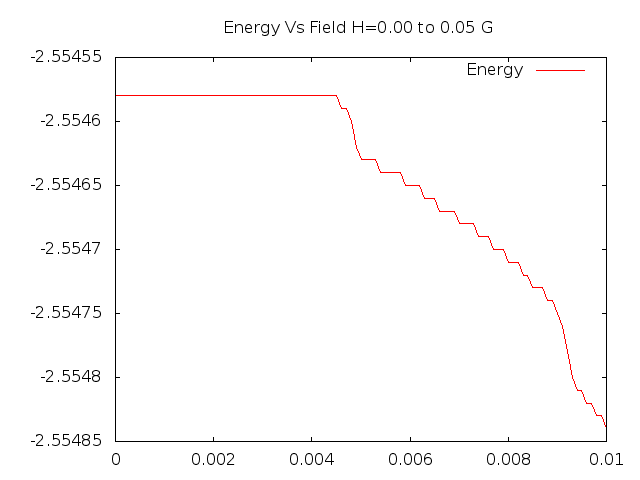
\includegraphics[scale=0.3]{E000to005G.png}
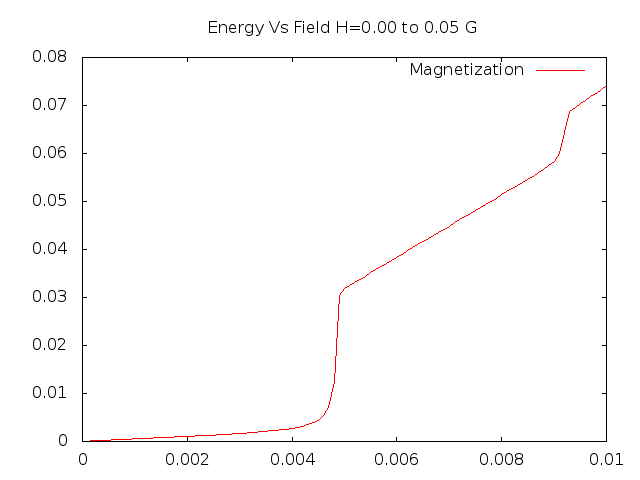
\includegraphics[scale=0.3]{M000to005G.png}
\caption{Energy vs increasing field and Magnetization versus increasing field}
\end{figure}
\begin{figure}[ht]
\centering
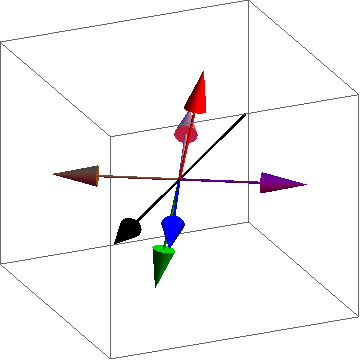
\includegraphics[scale=0.27]{1S000to005G.png}
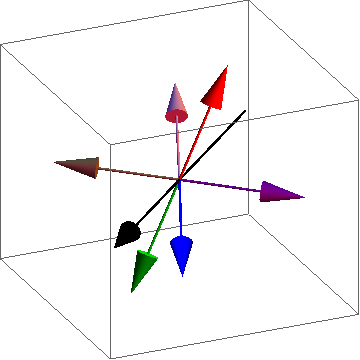
\includegraphics[scale=0.27]{47S000to005G.png}
\includegraphics[scale=0.27]{53S000to005G.png}
\includegraphics[scale=0.27]{83S000to005G.png}
\includegraphics[scale=0.27]{92S000to005G.png}
\includegraphics[scale=0.27]{98S000to005G.png}
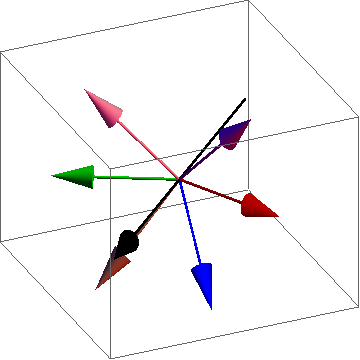
\includegraphics[scale=0.27]{501S000to005G.png}
\caption{Snapshots of the 6 characteristic spins of the lattice at H=0, 0.0046, 0.0052, 0.0082, 0.0091, 0.0097, and 0.05}
\end{figure}

\begin{figure}
\centering
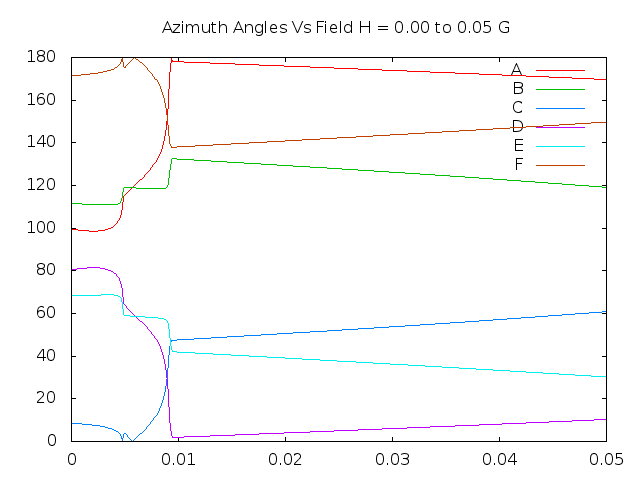
\includegraphics[scale=0.5]{azim000to005.png}
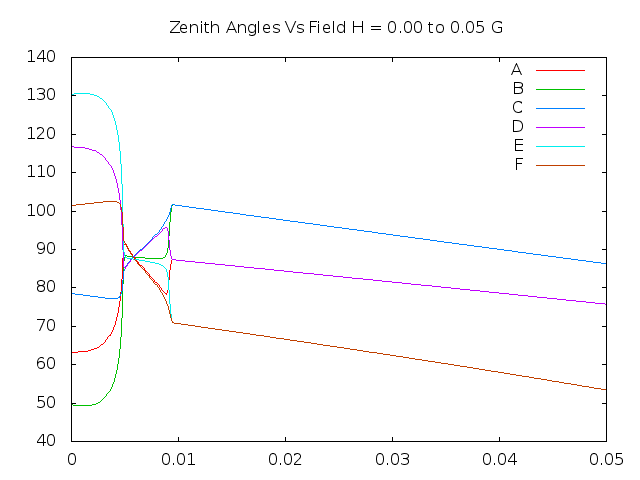
\includegraphics[scale=0.5]{zen000to005.png}
\caption{The angles are those between a chosen vector lying in the plane intersected by 111,
and a projection of each of the A, B, C, D, E, and F spins. Azimuthal angles are followed by zenith angles.}
\end{figure}

\begin{center}
\vspace*{\fill}
\begin{figure}
\includegraphics[keepaspectratio,scale=0.65]{Sfreq000to005G.png}
\caption{Peaks in the number of unique spins at approx. 0.05 and 0.09, indicating the occurence of transitions.}
\end{figure}
\vspace*{\fill}
\end{center}

\thispagestyle{plain}
\begin{center}
\LARGE
RUN 2: Decreasing Field, Ground State
\end{center}
\paragraph
\large
Similar to starting with a high field in the 111 direction, the spins are in a planar state that is
aligned with the field. When the field is lowered, the spins are stuck in a planar state. In the first
snapshot of the spins, the brown and green spins are partially aligned. This is likely due to insufficient
number of iterations for EFM. 3000 steps is typically sufficient, while 2000 is not. 
\begin{figure}[h]
 \centering 
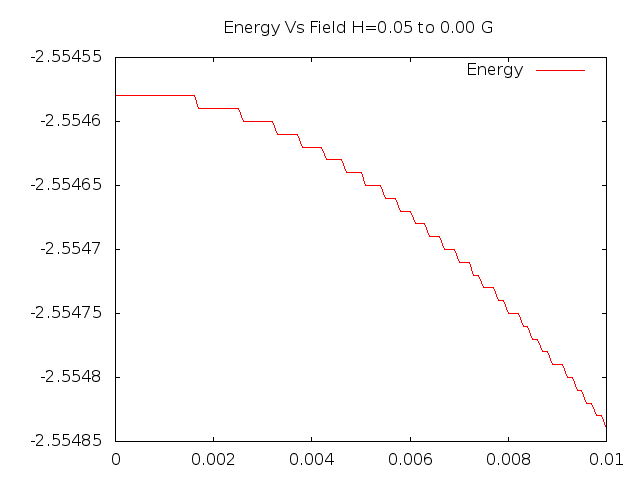
\includegraphics[scale=0.3]{E005to000G.png}
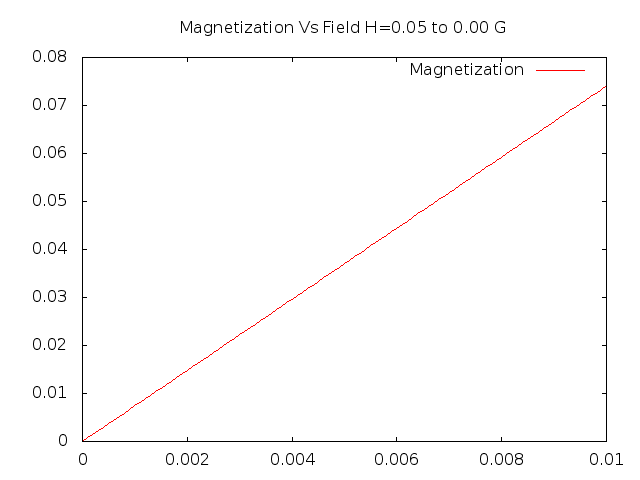
\includegraphics[scale=0.3]{M005to000G.png}
\caption{Energy vs decreasing field and Magnetization versus decreasing field}
\end{figure}
\begin{figure}[ht]
\centering
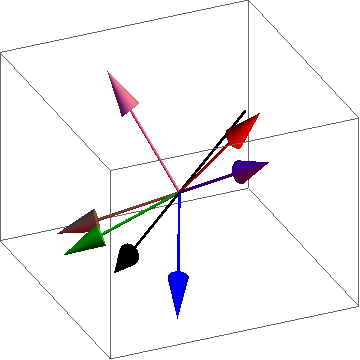
\includegraphics[scale=0.27]{1S005to000G.png}
\includegraphics[scale=0.27]{83S005to000G.png}
\includegraphics[scale=0.27]{344S005to000G.png}
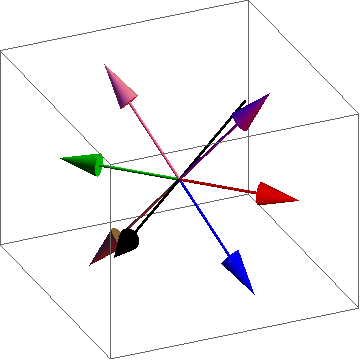
\includegraphics[scale=0.27]{501S005to000G.png}
\caption{Snapshots of the 6 characteristic spins of the lattice at B=0.05, B=0.0418, B=0.0157, and B=0.00}
\end{figure}

\begin{figure}
\centering
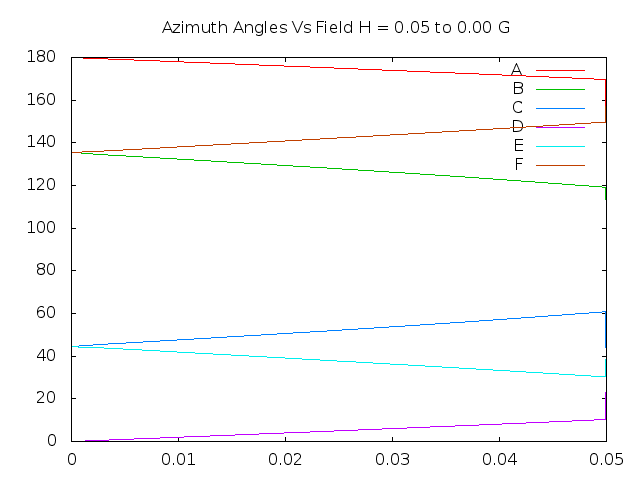
\includegraphics[scale=0.5]{azim005to000.png}
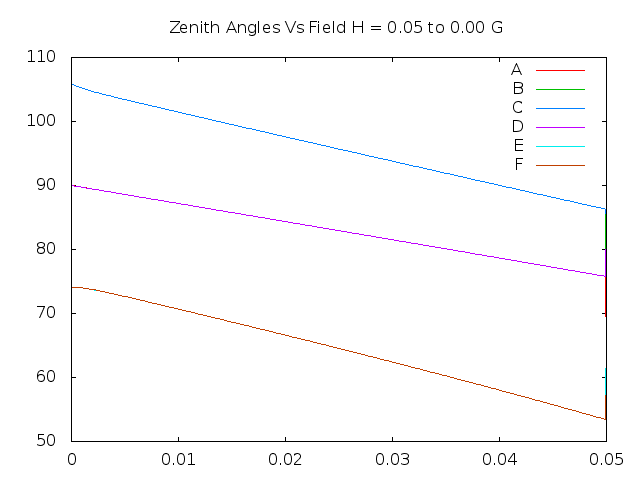
\includegraphics[scale=0.5]{zen005to000.png}
\caption{The angles are those between a chosen vector lying in the plane intersected by 111,
and a projection of each of the A, B, C, D, E, and F spins. Azimuthal angles are followed by zenith angles.}
\end{figure}

\begin{center}
\vspace*{\fill}
\begin{figure}
\centering
 \includegraphics[keepaspectratio,scale=0.65]{Sfreq005to000G.png}
 \caption{A peak in the number of unique spins at approx H = 0.007, yet no transition occurs in the lattice.}
\end{figure}
\vspace*{\fill}
\end{center}

\pagebreak 

\thispagestyle{plain}
\begin{center}
\LARGE
RUN 3: Increasing Field, Random State
\end{center}
\paragraph
\large
Very similar to run 1, in that there are 2 transitions at approximately 0.0038 and 0.0075. The transformation of the 
6 spins is similar as well,
with the spins beginning in the groundstate, transition to a planar state, 2 pairs of spins rotate and switch places,
and the plane the spins lie in reorients itself. The spins then gradually align with the field, and nothing
else interesting happens. 
\begin{figure}[h]
 \centering 
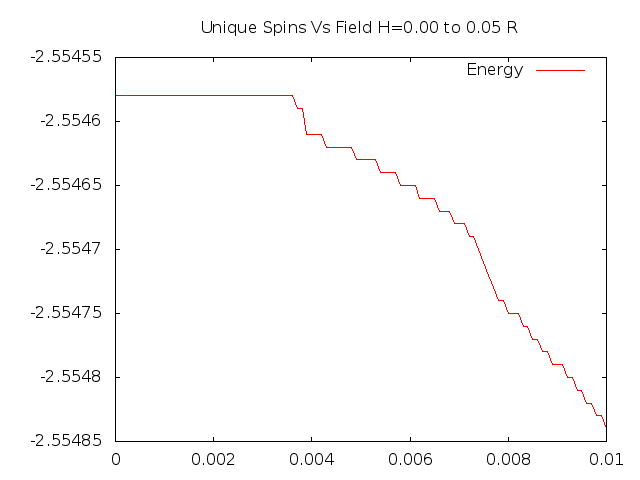
\includegraphics[scale=0.3]{E000to005R.png}
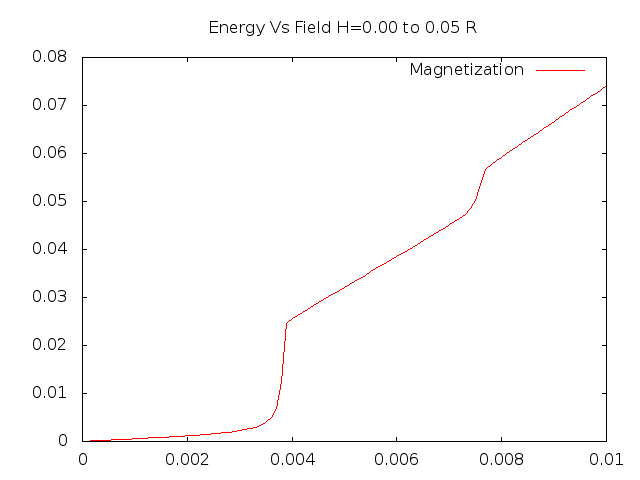
\includegraphics[scale=0.3]{M000to005R.png}
\caption{Energy vs increasing field and Magnetization versus increasing field}
\end{figure}
\begin{figure}[ht]
\centering
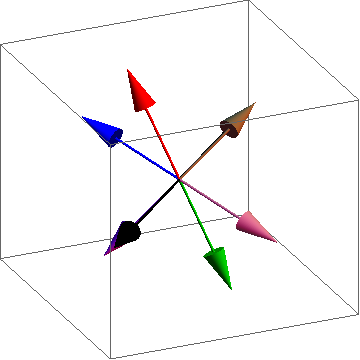
\includegraphics[scale=0.27]{1S000to005R.png}
\includegraphics[scale=0.27]{33S000to005R.png}
\includegraphics[scale=0.27]{42S000to005R.png}
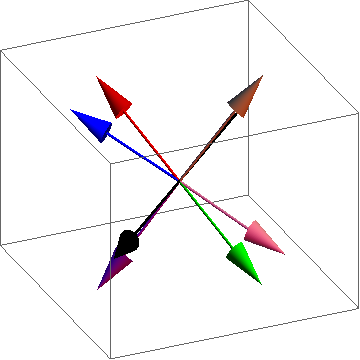
\includegraphics[scale=0.27]{69S000to005R.png}
\includegraphics[scale=0.27]{76S000to005R.png}
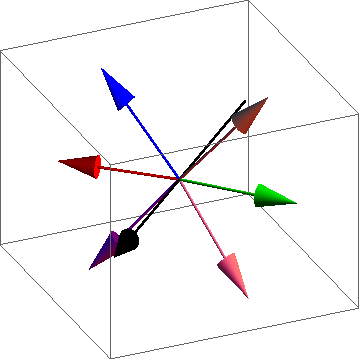
\includegraphics[scale=0.27]{82S000to005R.png}
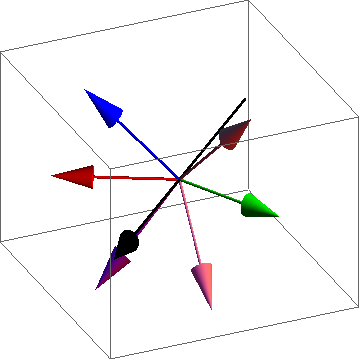
\includegraphics[scale=0.27]{501S000to005R.png}
\caption{Snapshots of the 6 spins at H = 0.00, 0.0032, 0.0041, 0.0068, 0.0075, 0.0081, and 0.05}
\end{figure}
\begin{figure}
\centering
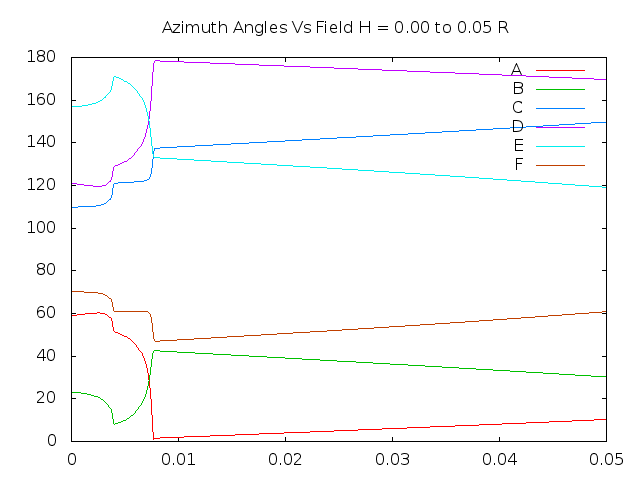
\includegraphics[scale=0.5]{azim000to005R.png}
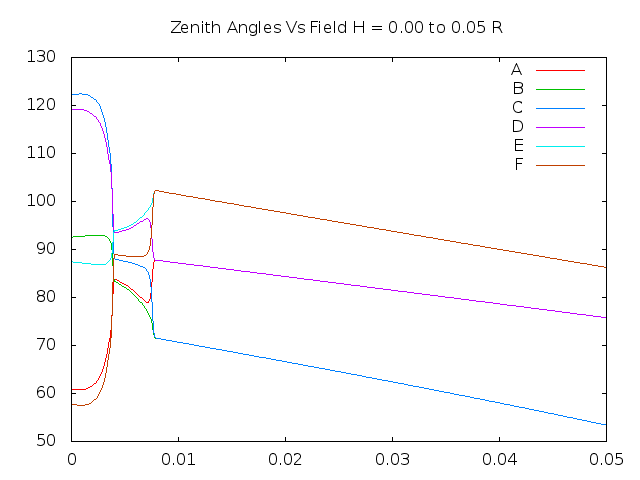
\includegraphics[scale=0.5]{zen000to005R.png}
\caption{The angles are those between a chosen vector lying in the plane intersected by 111,
and a projection of each of the A, B, C, D, E, and F spins. Azimuthal angles are followed by zenith angles.}
\end{figure}

\pagebreak

\begin{center}
\vspace*{\fill}
\begin{figure}
 \includegraphics[keepaspectratio,scale=0.65]{Sfreq000to005R.png}
 \caption{A peak in the number of unique spins occurs at approximately 0.0038 and 0.0075}
\end{figure}
\vspace*{\fill}
\end{center}
\pagebreak

\thispagestyle{plain}
\begin{center}
\LARGE
RUN 4: Decreasing Field, Random State
\end{center}
\paragraph
\large
A sudden transition occurs at approximately 0.022. The green and pink spins swap places with another, and the blue
and red spins also follow this swap. It's possible this transition only occurs because there is insufficient
steps being used for EFM, as was the case with applying the field in the 111 direction. Any transitions disappeared
when increasing the number of steps from 2000 to 3000 steps when decreasing the field with a random initial 
configuration. 
\begin{figure}[h]
 \centering 
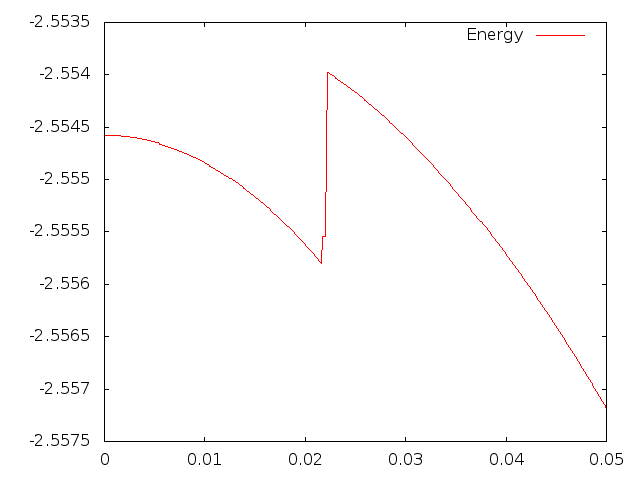
\includegraphics[scale=0.3]{E005to000R.png}
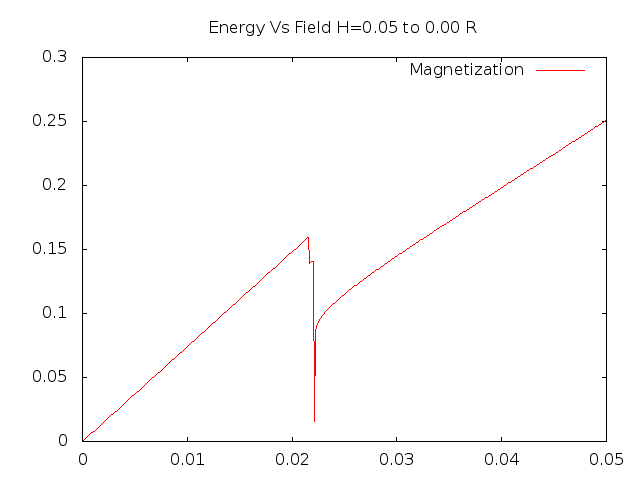
\includegraphics[scale=0.3]{M005to000R.png}
\caption{Energy vs decreasing field and Magnetization versus decreasing field}
\end{figure}
\begin{figure}[ht]
\centering
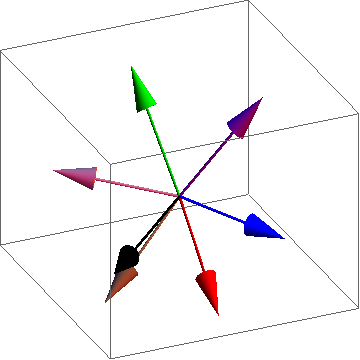
\includegraphics[scale=0.23]{1S005to000R.png}
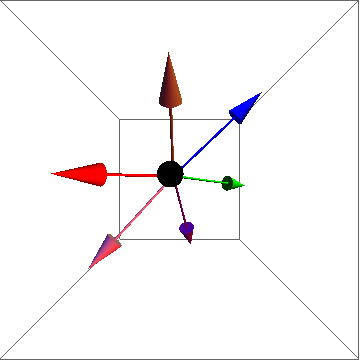
\includegraphics[scale=0.23]{244S005to000R.png}
\includegraphics[scale=0.23]{277S005to000R.png}
\includegraphics[scale=0.23]{280S005to000R.png}
\includegraphics[scale=0.23]{281S005to000R.png}
\includegraphics[scale=0.23]{283S005to000R.png}
\includegraphics[scale=0.23]{284S005to000R.png}
\includegraphics[scale=0.23]{285S005to000R.png}
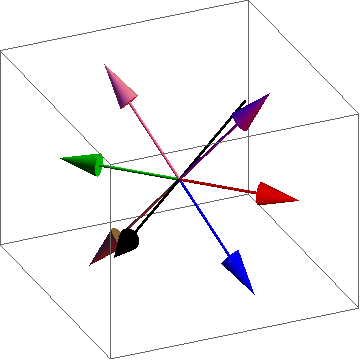
\includegraphics[scale=0.23]{501S005to000R.png}
\includegraphics[scale=0.23]{501AltS005to000R.png}
\caption{Snapshots of the 6 characteristic spins at H = 0.05, 0.0257, 0.0224, 0.0221, 0.0220, 0.0218, 0.0217, 0.0216
and 0.00. An alternate view of the spins at H = 0.00 is also shown.}
\end{figure}

\begin{figure}
\centering
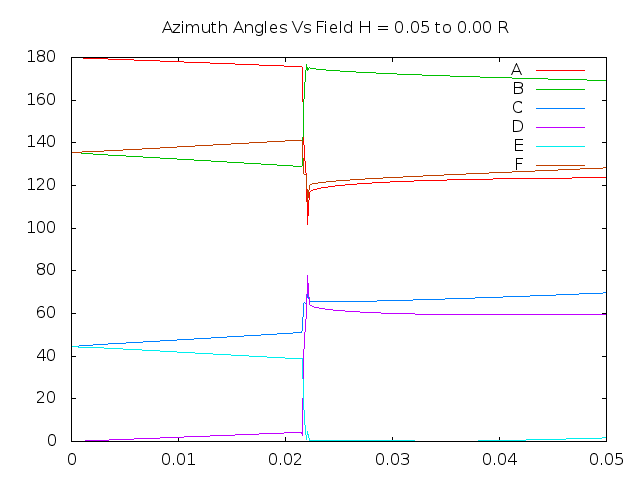
\includegraphics[scale=0.5]{azim005to000R.png}
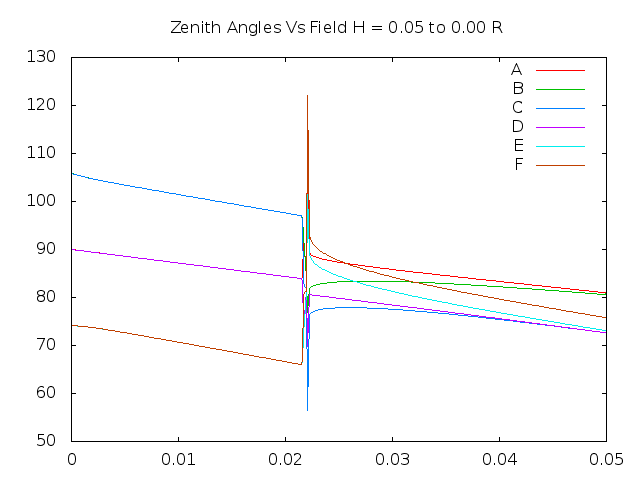
\includegraphics[scale=0.5]{zen005to000R.png}
\caption{The angles are those between a chosen vector lying in the plane intersected by 111,
and a projection of each of the A, B, C, D, E, and F spins. Azimuthal angles are followed by zenith angles.}
\end{figure}

\begin{center}
\begin{figure}
 \includegraphics[keepaspectratio,scale=0.65]{Sfreq005to000R.png}
 \caption{The lattice is highly disordered from H = 0 to H = 0.029. A six spin system is finally achieved after
 this point.}
\end{figure}
\end{center}

\pagebreak
\LARGE\textbf{\centering Appendices} \\
\Large
Appendix A - Finding Unique Spins
\large
\paragraph{Overview}
The azimuth angles are found by projecting each of the 6 chosen spins into the 111 plan and dotting the projections
with the (1,-1,0) vector; a vector that lies in the 111 plane. The zenith angles are found by dotting each of the
spins with the 111 normal vector. 
\end{document}